% ============================================================
%  Relative Performance Feedback and Redistribution Preferences
%  Isabella Valencia — Paris School of Economics
%  Working Paper, May 2026
% ============================================================
\documentclass[12pt]{article}

\usepackage[margin=1in]{geometry}
\usepackage{setspace}
\usepackage{booktabs}
\usepackage{amsmath}
\usepackage{graphicx}
\usepackage{hyperref}
\usepackage{natbib}
\usepackage{caption}
\usepackage{subcaption}
\usepackage[T1]{fontenc}
\usepackage{lmodern}
\usepackage{tabularray}
\usepackage{siunitx}
\usepackage{xcolor}
\UseTblrLibrary{booktabs}

\hypersetup{colorlinks=true, linkcolor=black, citecolor=black, urlcolor=blue}
\onehalfspacing

% ============================================================
\begin{document}

\title{\textbf{Relative Performance Feedback and Redistribution Preferences:
Evidence from an Online Experiment}\thanks{
This experiment builds on the design of \citet{Almas2020} and is inspired
by the research question of \citet{Cassar2019}.}}

\author{Isabella Valencia\\
\small Paris School of Economics\\
\small \href{mailto:valenciaisabellap@gmail.com}{valenciaisabellap@gmail.com}}

\date{May 2026}

\maketitle

% ============================================================
\begin{abstract}
\noindent
This paper examines how relative performance feedback affects redistribution
preferences and beliefs about effort versus luck in generating inequality.
In an online experiment, participants complete a code-recognition task and
are randomly assigned to one of three conditions: no feedback, told they
performed \emph{above} a randomly matched peer, or told they performed
\emph{below}.
They then act as impartial spectators and redistribute a fixed sum between
two workers whose earnings reflect their performance.
Participants told they outperformed their peer score 1.23 points higher on
an effort-attribution scale (0--10) than those told they underperformed
($p < 0.05$) and redistribute \$0.52--0.55 less to the lower-earning worker
($p < 0.10$).
The no-feedback group sits between the two treatment arms; neither its
belief score nor its redistribution differs significantly from either
treated group.
A mediation analysis shows that roughly 50 percent of the redistribution
effect is explained by the shift in effort--luck beliefs, consistent with
self-serving attribution as the channel linking feedback to redistribution.
\end{abstract}

\bigskip
\noindent\textbf{Keywords:} redistribution, relative performance feedback,
self-serving attribution, fairness, online experiment\\
\noindent\textbf{JEL codes:} C91, D31, D63, D91

\newpage

% ============================================================
\section{Introduction}

Free-market economies inherently generate unequal outcomes, and while modern
democratic societies rely on redistribution to mitigate these disparities,
there is persistent disagreement over which inequalities are considered
legitimate \citep{AlesinGiulian2011, Piketty2014}.
A central dimension of this debate concerns the \emph{source} of inequality:
outcomes attributed to effort are typically viewed as more deserving than those
arising from luck.
This intuition is formalised in the accountability framework, which models
redistributive preferences as judgments about deservingness and predicts lower
redistribution when inequality reflects effort rather than chance
\citep{Konow2000, Cappelen2007}.
The framework finds broad empirical support: beliefs about the determinants of
income are consistently among the strongest predictors of redistribution
preferences \citep{Piketty1995, Alesina2005, Benabou2006}.

Yet a key difficulty in this debate is that, in practice, the source of
inequality is rarely clear-cut.
Individual success reflects a mix of effort, innate ability, family
background, and circumstance, and it is often hard to separate these
contributions, even for the person directly involved \citep{Piketty2014}.
When effort and luck cannot be cleanly distinguished, beliefs about which
is responsible do not simply reflect the available evidence; they are also
shaped by personal experience and motivated reasoning \citep{Kunda1990}.
Since these beliefs drive redistribution preferences, whatever shapes them
also shapes redistribution demand.

\citet{Deffains2016} argue that the experience of success and failure
shapes redistribution preferences through the self-serving bias:
individuals who succeed at a task attribute their outcome to effort and
favour less redistribution, while those who fail attribute their outcome
to circumstance and shift toward more.
Since wealthier individuals have typically experienced more success, this
bias systematically pushes them to view inequality as earned rather than
lucky, creating a divide between rich and poor not just in material
interests but also in fairness views.
As \citet{Deffains2016} put it, wealthy individuals ``do not only oppose
redistribution because they expect to be net payers, but also because the
self-serving bias systematically shifts their fairness principles.’’
Identifying this channel outside a controlled setting is difficult, however:
in observational data one cannot tell whether successful individuals
attribute outcomes to effort because of cognitive bias or because they
genuinely worked harder.
Isolating the self-serving bias therefore requires exogenous variation in
comparative signals, holding actual performance constant while shifting
only what individuals learn about their relative standing.
This paper asks whether such a signal --- being told one outperformed or
underperformed a peer --- is enough to shift beliefs about the role of
effort in generating inequality and, through that channel, redistribution
preferences.

This paper provides experimental evidence on this mechanism.
Participants complete a performance task and are randomly assigned to one of
three conditions: (i) \emph{no feedback} about relative standing; (ii) told
they performed \emph{above} a randomly matched peer (\emph{above} group);
or (iii) told they performed \emph{below} a matched peer (\emph{below}
group).
Subsequently, all participants act as impartial spectators and decide how to
distribute a fixed monetary sum between two workers whose inequality arose
from differential performance.

The key findings are three.
First, participants told they outperformed a peer redistribute less in the
merit scenario: \$1.91 on average, versus \$2.44 in the below group and
\$2.12 in the no-feedback group.
The above--below gap of \$0.52--0.55 is marginally significant ($p < 0.10$)
across both specifications.
Second, the same group scores 1.23 points higher on an effort-attribution
scale (0--10) than the below group ($p < 0.05$), consistent with
self-serving belief updating; the joint test across all three groups also
rejects equality of means ($p = 0.039$, ANOVA).
\begingroup\color{red}\bfseries
Third, neither treatment arm individually differs significantly from the
no-feedback group; the significant contrast is the above--below gap.
This is consistent with both signals pushing beliefs in opposite directions
from a common baseline, rather than one side driving the effect
asymmetrically.
Together, these results suggest that receiving a comparative signal ---
in either direction --- shifts effort attribution and redistribution
relative to receiving no signal, with the two treated groups diverging
significantly from each other.

These results are consistent with the self-serving attribution account of
redistribution developed by \citet{Deffains2016}: individuals who perform
well relative to others update their beliefs about the role of effort in
generating inequality and become less redistributive.
Our design extends their framework by using randomly assigned comparative
feedback, providing clean causal identification and isolating the relative
rather than absolute performance channel.
One notable difference is that \citet{Deffains2016} find SSB effects on
both sides --- success reduces redistribution and failure increases it ---
whereas our evidence is concentrated on the winning side.
The absence of a significant response among participants told they
underperformed suggests that the SSB in our setting is more asymmetric:
learning one beat a peer is enough to trigger meritocratic updating, but
learning one lost does not produce a symmetric shift toward redistribution.
The paper most directly relates to \citet{Almas2020}, from whose spectator
design we adapt the merit redistribution task, and to \citet{Cassar2019},
whose focus on how performance comparisons shape distributive preferences
motivates our research question.
Our contribution is to provide clean experimental identification of the
direction and asymmetry of this effect using randomly assigned relative
feedback. [REVISAR: confirmar asimetría con test lineal below vs.\
no-feedback antes de finalizar.]
\endgroup

The rest of the paper is structured as follows.
Section~\ref{sec:lit} reviews the related literature.
Section~\ref{sec:design} describes the experimental design.
Section~\ref{sec:results} presents the results.
Section~\ref{sec:conclusion} concludes.

% ============================================================
\section{Related Literature}
\label{sec:lit}

This paper contributes to three strands of literature.

\paragraph{Beliefs about inequality and redistribution.}
A key insight from \citet{Piketty1995} is that beliefs about social
mobility and the role of effort versus luck determine preferences for
redistribution in equilibrium.
\citet{Alesina2005} provide empirical evidence: Americans attribute poverty
more to individual failure than Europeans, which partly explains the
cross-country gap in redistribution.
\citet{Benabou2006} model how self-serving motivated reasoning sustains
two equilibria --- a ``belief in a just world'' and a more luck-oriented view
--- with different steady-state redistribution levels.
Our experiment directly tests the mechanism by which an informational shock
(relative performance feedback) updates beliefs and behaviour.

\paragraph{Impartial spectator and fairness views.}
\citet{Cappelen2007} and \citet{Cappelen2013} use spectator designs to
classify subjects into fairness types (libertarian, meritocratic, egalitarian)
and show that a majority of individuals prefer some redistribution away from
inequality that arises from luck rather than effort.
We adapt their spectator design to a merit scenario and ask whether
third-party redistribution decisions are affected by information about the
spectator's own relative performance --- a test of whether the spectator role
is truly impartial.

\paragraph{Self-serving attribution and social comparisons.}
Self-serving attribution refers to the tendency to attribute successes
internally (effort) and failures externally (luck or circumstance)
\citep{Miller1975, Mezulis2004}.
In an economic context, \citet{Babcock1995} document that parties in
bargaining inflate self-assessments of a fair outcome in a self-serving
direction.
Closer to our design, \citet{Deffains2016} show that individuals who
experience unfair treatment become more supportive of redistribution.
\citet{Cassar2019} show that framing one's own performance as a failure
(relative to a counterfactual) shapes distributive preferences; our design
extends this insight by using randomly assigned comparative feedback,
allowing clean causal identification.
We add to this literature by focusing on the \emph{comparative} and
\emph{asymmetric} dimension: the same absolute performance level can produce
different attribution and redistribution depending on whether one learns one
stands above or below a peer, and the effect appears concentrated on the
winning side.

% ============================================================
\section{Experimental Design}
\label{sec:design}

The experiment was conducted online using JATOS and hosted the free, ESCoP-sponsored server Mindprobe.
The whole design  builds on the spectator design of \citet{Almas2020}.
It involved two distinct roles: \emph{workers} and \emph{spectators}.

\textbf{Workers} ($n = 2$) were recruited through Prolific and completed the
code-recognition task under real monetary incentives.
They were paid a base fee of \$4 plus a performance-based bonus of up to \$8,
for a maximum possible payout of \$12 each.
They were informed in advance that their earnings would initially depend on
their relative performance against each other---the higher-scoring worker
would receive \$8 while the other would receive \$0---and that a third party
(a spectator) would subsequently decide whether and how much to redistribute
between them.

\textbf{Spectators} ($n = 134$) were recruited through personal networks
(friends, family, and colleagues from two workplaces), completed the full
experiment online in approximately 10 minutes, and received no monetary
compensation.
The experiment consisted of two parts: a code-recognition task and a
redistribution decision task in which they acted as impartial spectators.
Spectators were informed before making their redistribution decisions that the
workers were real individuals who had completed the same task and would
receive actual monetary payouts determined by one randomly selected
spectator's allocation.
The impartial-spectator design thus removes material self-interest on the
spectator side while keeping real stakes for the workers, ensuring that
decisions have genuine consequences and giving the design greater external
validity.

\subsection{Part 1: Code-Recognition Task}

Participants (both workers and spectators) completed a code-recognition task
consisting of one practice round of 20~seconds followed by five scored rounds
of 45~seconds each.
At the start of each round, a three-digit target number (drawn from 100--999)
was displayed at the top of the screen.
Below it, a grid of three-digit numbers appeared; approximately 15 percent
of the codes in the grid matched the target (around 48 instances per round),
and the rest were distractors.
Participants had to identify and check every instance of the target as
quickly as possible.
The grid was generated randomly at the start of each round, so the target
and distractor codes changed every 45~seconds.
To ensure a consistent interface experience, the grid dimensions were
adapted to screen size: desktop users saw a $20 \times 16$ grid (320~codes),
while mobile users saw a $7 \times 46$ grid (322~codes), with the same
number of target instances in both cases.
Participants were explicitly told about the scoring system: they earned
1~point for each correct identification, lost 1~point for each false alarm,
and received no penalty for a missed target.
The maximum possible score across the five rounds was around 200~points; sample
means range from 90 to 95 points across treatment groups
(Table~\ref{tab:balance}).\footnote{This marked the end of the task for
the two workers. Before exiting, they were reminded that one spectator,
chosen at random, would decide how to split their earnings, and that this
decision would be paid out as their bonus. Spectators continued to Part~2,
as described bellow.}

Just after finishing, participants answered three pre-feedback self-report
questions: (i) effort exerted (slider, 0--10); (ii) guessed score (numeric,
range $-200$ to $200$); and (iii) relative performance prediction
(``I would perform better than or the same as the other participant''
vs.\ ``I would perform worse'').

\subsection{Treatments: Relative Performance Feedback}
\label{sec:treatments}

After the self-report, participants were randomly assigned to one of three
feedback conditions.

\begin{enumerate}
  \item \textbf{No feedback.} Participants were informed they could proceed to
    Part~2 without seeing their score or any comparison information.
  \item \textbf{Above.} Participants were told:
    ``You performed above your randomly matched peer.''
  \item \textbf{Below.} Participants were told:
    ``You performed below your randomly matched peer.''
\end{enumerate}

The feedback signal was generated through a dynamic matching procedure.
Before the main data collection, ten pilot participants completed the task,
providing an initial distribution of scores and establishing a current best
and worst performer.
As each subsequent spectator completed the task, those randomly assigned to
the \emph{above} condition were matched with the current lowest scorer in the
spectator pool; those assigned to the \emph{below} condition were matched
with the current highest scorer.
Reference scores were updated continuously as the experiment progressed.
Note that spectators were compared with other spectators in this pool and 
the matching was indeed random. This design guarantees genuine, non-deceptive 
feedback: every participant in
the above condition truly outperformed their assigned reference peer, and
every participant in the below condition truly underperformed theirs.
Participants who could not receive their assigned treatment --- above-condition
participants who scored below the current worst, or below-condition
participants who scored above the current best --- were excluded from the
analysis.
At debriefing, participants were shown their actual score and informed of the
matching procedure, so they could understand why they had received the message
they did.

\subsection{Part 2: Distribution Decisions}
\label{sec:distdecisions}

After the (non)feedback screen, all participants acted as impartial spectators and
made a redistribution decision adapted from \citet{Almas2020}.

\subsubsection*{Redistributive Decision in a Merit Scenario}

Participants read that two real participants --- the two workers who had
previously completed the same task --- were identified as Worker~A and
Worker~B.
Worker~A had received a larger initial payment because they performed better;
Worker~B received nothing because they performed worse.
Participants were asked to decide whether and how to redistribute the given endowment
between the two workers.
The decision was presented as a set of discrete options covering
the full range from keeping full inequality to reversing it.

After the redistribution decision, participants completed a short demographics
survey (age, gender, and education) followed by the key belief measure of
this study.
They were asked to respond to the following question using a slider:

\begin{quote}
\textit{``To what extent do you think the initial income (before any redistribution) of the participants
in the previous task was determined by effort versus luck?''}
\end{quote}

\noindent The slider ranged from 0 (``Completely determined by luck'') to
10 (``Completely determined by effort'').
This variable (\texttt{effort\_luck}) is the hypothesised mediator between
relative performance feedback and redistribution preferences.

\subsection{Key Outcome and Mediator Variables}

\begin{itemize}
  \item \textbf{Redistribution (merit):} USD allocated to Worker~B in the
    merit scenario. Primary outcome variable.
  \item \textbf{Effort--luck belief (\texttt{effort\_luck}):} Score on the
    0--10 slider described above. Hypothesised mediator.
\end{itemize}

\subsection{Sample}

Spectators were recruited through personal networks: friends, family, and
employees at two workplaces.
The analysis sample consists of $N = 145$ spectators after excluding
non-engagers (zero score and zero clicks).
The sample is predominantly Colombian (76.5\%), with the remainder drawn from
other countries, primarily in Europe.
As this is a convenience sample, findings should be interpreted with caution
regarding external validity and may not generalise to other populations in
terms of magnitudes; treatment assignment was, however, random within this
sample, so internal validity is preserved.

Table~\ref{tab:balance} presents descriptive statistics by treatment group.
Groups are balanced on all pre-determined covariates: age ($p = 0.94$),
gender ($p = 0.57$), task score ($p = 0.71$), nationality ($p = 0.32$),
and education ($p = 0.52$), confirming that randomisation was successful.
The nationality variable shows the above group with a slightly higher share
of Colombians (83\%) compared to the no-feedback (70\%) and below (77\%)
groups, though this difference is comfortably non-significant ($p = 0.32$)
and attributable to chance given the small sample size.

The effort--luck belief score differs significantly across groups ($p = 0.039$),
which is itself a key outcome; importantly, this measure is elicited
\emph{after} the feedback treatment, so it cannot confound treatment
assignment.

\begin{table}[!h]
\centering
\caption{Descriptive Statistics by Treatment Group \label{tab:balance}}
\centering
\begin{tabular}[t]{lllll}
\toprule
 & Told: Above & No Feedback & Told: Below & $p$-value\\
\midrule
Task score & 91.26 (17.63) & 94.84 (20.77) & 91.06 (26.89) & 0.640\\
Age & 34.87 (13.62) & 35.39 (14.78) & 34.70 (14.67) & 0.971\\
Female (\%) & 59.57 (49.61) & 61.22 (49.23) & 70.21 (46.23) & 0.513\\
Colombian (\%) & 80.85 (39.77) & 69.39 (46.57) & 76.60 (42.80) & 0.417\\
Predicted above average (\%) & 89.36 (31.17) & 87.76 (33.12) & 78.72 (41.37) & 0.290\\
\addlinespace
Education (\%) &  &  &  & 0.484\\
\quad Less than bachelor & 23.40 (42.80) & 18.37 (39.12) & 10.64 (31.17) & \\
\quad Bachelor's & 48.94 (50.53) & 48.98 (50.51) & 61.70 (49.14) & \\
\quad Master's or above & 27.66 (45.22) & 32.65 (47.38) & 27.66 (45.22) & \\
$N$ & 47 & 49 & 47 & 143\\
\bottomrule
\multicolumn{5}{l}{\textsuperscript{} Mean (SD) for continuous variables; mean $\times$ 100 (SD $\times$ 100) for binary. $p$-values}\\
\multicolumn{5}{l}{from one-way ANOVA (continuous) or chi-squared test (binary). Predicted above average: share}\\
\multicolumn{5}{l}{expecting to outperform matched peer, elicited before feedback.}\\
\end{tabular}
\end{table}


% ============================================================
\section{Results}
\label{sec:results}

\begin{figure}[h!]
\centering
\caption{Effort Attribution and Merit Redistribution by Treatment Group}
\label{fig:main}
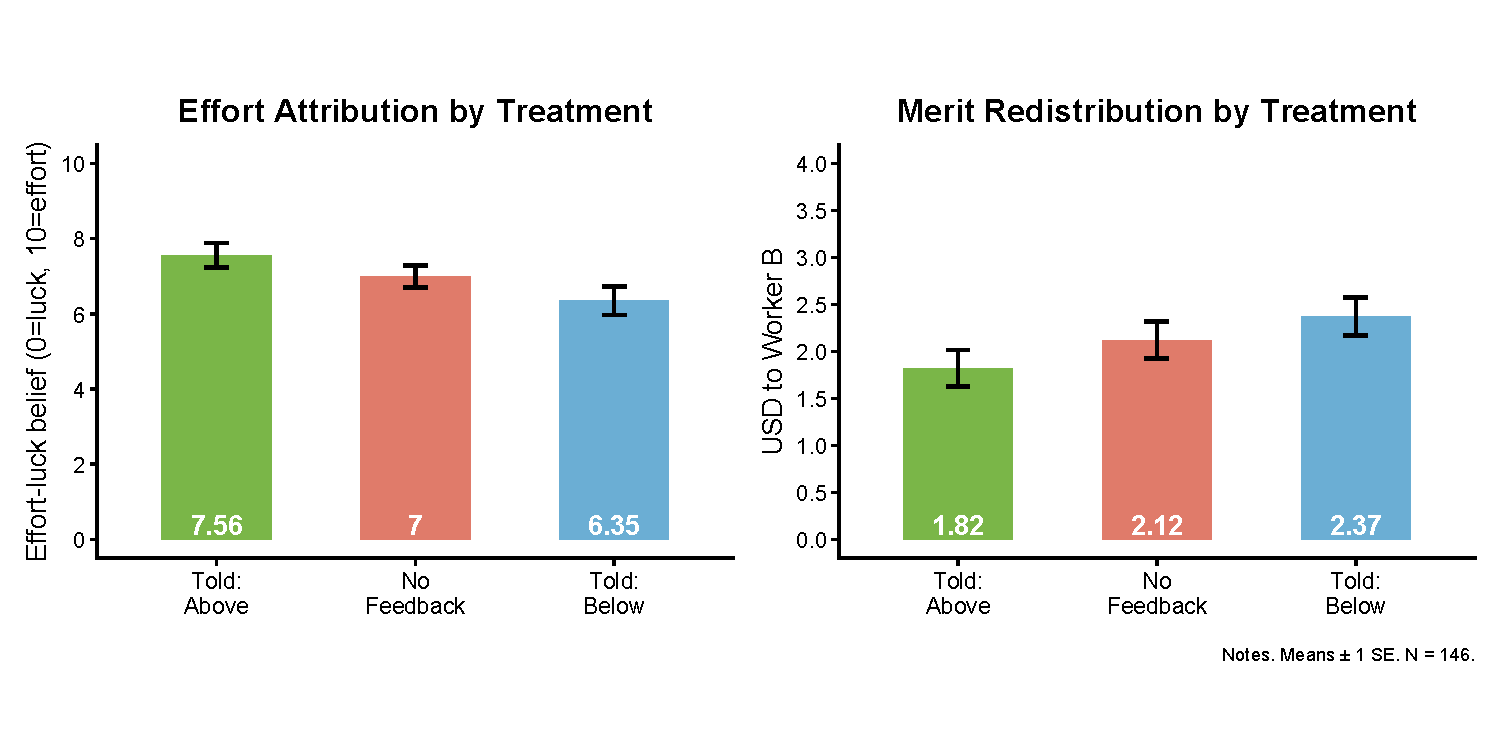
\includegraphics[width=\textwidth]{figure2.pdf}
\vspace{4pt}
\footnotesize\textit{Notes.}
Left panel: mean effort--luck belief (0 = 100\% luck; 10 = 100\% effort),
elicited after the redistribution decision.
Right panel: mean USD allocated to the lower-earning worker (merit scenario).
Bar heights are group means; whiskers are $\pm 1$ SE. $N = 145$.
\end{figure}

Figure~\ref{fig:main} gives an overview of both main outcomes across
the three treatment arms.
Among the 145 spectators in the sample, 47 were told they outperformed their
matched peer (above), 48 were told they underperformed (below), and 50
received no feedback.
The left panel shows mean effort--luck belief and the right panel shows mean
redistribution to the lower-earning worker; both outcomes display the same
monotone gradient.
The above group attributes the most to effort and redistributes the least;
the below group is the most luck-oriented and the most redistributive; and
the no-feedback group sits between the two.
The most salient visual feature in both panels is the above--below gap: the
distance between the two treated groups is roughly twice the distance of
either group from the no-feedback anchor.
By contrast, the no-feedback group sits close to the midpoint, and neither
treated group differs from it by a large margin individually --- a pattern
consistent with both signals pushing in opposite directions from a common
baseline, with the joint above--below contrast being the statistically
identifiable effect.

\subsection{Effort--Luck Beliefs}
\label{sec:beliefs}

The left panel shows a clear monotone pattern: the above group scores highest
($\overline{EL}_{\text{above}} = 7.48$, SD = 2.36), followed by the
no-feedback group ($\overline{EL}_{\text{nofb}} = 7.00$, SD = 2.03) and
the below group ($\overline{EL}_{\text{below}} = 6.24$, SD = 2.57).
Notably, all three groups score above the scale midpoint of 5, indicating
that effort attribution is the modal view regardless of treatment; what
the feedback shifts is the \emph{degree} to which participants see the
outcome as effort-determined.
A one-way ANOVA rejects equality of group means ($p = 0.039$).

Columns 1--2 of Table~\ref{tab:main} report OLS regressions of the
effort--luck belief on treatment dummies, with the above group as the
baseline.
Without controls (column~1), the below group scores 1.23 points lower than
the above group (SE = 0.52, $p < 0.05$).
The no-feedback group scores 0.48 points lower (SE = 0.46, $p = 0.30$),
roughly half the magnitude of the below-group gap and not statistically
significant, consistent with the absence of any comparative signal that
would activate motivated attribution.
Taking the no-feedback group as a natural anchor, the point estimates suggest
that positive feedback elevates effort attribution by roughly 0.48 points
above this anchor, while negative feedback depresses it by approximately
0.76 points below it --- both signals moving in the expected direction,
though neither individual shift is large enough to be statistically
significant on its own.
Once controls are added (column~2), both estimates remain stable: the
below-group gap widens slightly to 1.34 points (SE = 0.53, $p < 0.05$),
and the no-feedback coefficient is $-0.50$ (SE = 0.46), confirming that
the pattern does not reflect pre-existing compositional differences across
groups.

These findings are consistent with the motivated-reasoning account of
\citet{Kunda1990}: positive comparative signals are more readily
internalised because they serve the motivated goal of maintaining a
positive self-image, while negative signals invite counter-argument and
discounting \citep{Mezulis2004}.
Because the comparative signal is exogenously assigned and uncorrelated
with actual task performance, these belief differences cannot be explained
by genuine differences in effort across groups, providing experimental
support for the belief-updating channel theorised by \citet{Deffains2016}.

\subsection{Redistribution in the Merit Scenario}
\label{sec:merit}

The right panel shows mean redistribution following the same gradient.
The above group allocates the least (\$1.91, SD = \$1.35), followed by
the no-feedback group (\$2.12, SD = \$1.39) and the below group
(\$2.44, SD = \$1.38).
The one-way ANOVA yields $p = 0.179$, not significant at the omnibus
level, consistent with the gap being driven mainly by the above--below
contrast rather than uniform differences across all three groups.

Columns 3--4 of Table~\ref{tab:main} report the main OLS regressions
($N = 145$).
Without controls (column~3), the below group redistributes \$0.52 more
than the above group (SE = \$0.28, $p < 0.10$), while the no-feedback
group redistributes \$0.21 more (SE = \$0.28), a difference that is not
statistically significant.
With the full set of controls (column~4), the below-group estimate is
\$0.55 (SE = \$0.31, $p < 0.10$), remaining marginally significant.
The coefficient on the Colombian indicator is $-\$0.40$ (SE = \$0.30),
negative but not statistically significant; nationality is balanced
across treatment arms ($p = 0.32$), so this does not confound the
treatment comparison.

The above--below gap of \$0.52--0.55 is stable across specifications and
economically meaningful, representing roughly 27--29\% of the above-group
mean of \$1.91, and remains marginally significant in both columns.

\begin{table}
\centering
\begin{talltblr}[         %% tabularray outer open
caption={Treatment Effects on Effort Attribution and Redistribution \label{tab:main}},
note{}={* p \num{< 0.1}, ** p \num{< 0.05}, *** p \num{< 0.01}},
note{ }={\textit{Notes.} OLS with HC3-robust SEs in parentheses. Baseline: Told Above. Cols.~(1)--(2): effort--luck belief (0 = luck, 10 = effort). Cols.~(3)--(4): USD redistributed to lower-earning worker (merit scenario). Controls: age, female indicator, Colombian indicator, task score, and education (Less than bachelor = baseline). $^{*}p<0.10$, $^{**}p<0.05$, $^{***}p<0.01$.},
]                     %% tabularray outer close
{                     %% tabularray inner open
colspec={Q[]Q[]Q[]Q[]Q[]},
hline{2}={1-5}{solid, black, 0.05em},
hline{20}={1-5}{solid, black, 0.05em},
hline{1}={1-5}{solid, black, 0.08em},
hline{23}={1-5}{solid, black, 0.08em},
column{2-5}={}{halign=c},
column{1}={}{halign=l},
}                     %% tabularray inner close
& (1) & (2) & (3) & (4) \\
Constant & \num{7.442}*** & \num{6.542}*** & \num{1.957}*** & \num{3.614}*** \\
& (\num{0.358}) & (\num{1.343}) & (\num{0.199}) & (\num{0.820}) \\
No Feedback & \num{-0.446} & \num{-0.452} & \num{0.163} & \num{0.106} \\
& (\num{0.463}) & (\num{0.463}) & (\num{0.281}) & (\num{0.285}) \\
Told: Below & \num{-1.144}** & \num{-1.259}** & \num{0.448} & \num{0.466} \\
& (\num{0.524}) & (\num{0.535}) & (\num{0.284}) & (\num{0.305}) \\
Age &  & \num{0.019} &  & \num{-0.008} \\
&  & (\num{0.018}) &  & (\num{0.012}) \\
Female &  & \num{0.349} &  & \num{-0.284} \\
&  & (\num{0.423}) &  & (\num{0.237}) \\
Colombian &  & \num{0.350} &  & \num{-0.469} \\
&  & (\num{0.572}) &  & (\num{0.290}) \\
Task score &  & \num{-0.007} &  & \num{-0.006} \\
&  & (\num{0.009}) &  & (\num{0.006}) \\
Bachelor's degree &  & \num{0.428} &  & \num{-0.334} \\
&  & (\num{0.561}) &  & (\num{0.365}) \\
Master's or above &  & \num{0.515} &  & \num{-0.352} \\
&  & (\num{0.609}) &  & (\num{0.407}) \\
$N$ & \num{140} & \num{140} & \num{143} & \num{143} \\
$R^{2}$ & \num{0.039} & \num{0.099} & \num{0.018} & \num{0.076} \\
Controls (age, female, score, Colombian, edu.) & No & Yes & No & Yes \\
\end{talltblr}
\end{table}


\subsection{The Belief Channel: Mediation Analysis}
\label{sec:surprise}

If self-serving attribution is the mechanism at work, then the treatment
effect on redistribution should operate \emph{through} the effort--luck
belief.
Table~\ref{tab:mechanism} tests this by adding the effort--luck belief score
as a covariate to the redistribution regression.

Columns 1--2 of Table~\ref{tab:mechanism} use the full sample ($N = 142$,
three participants missing the belief slider and one the redistribution
decision).
The effort--luck belief score is a strong and highly significant predictor of
redistribution: each one-point increase on the 0--10 scale is associated with
\$0.20 less redistributed to the lower-earning worker (SE = \$0.05,
$p < 0.01$), both with and without additional controls.
Once effort--luck belief is included, the treatment coefficients become small
and statistically indistinguishable from zero: the below-group coefficient
falls from \$0.52 (column~3 of Table~\ref{tab:main}) to \$0.26
(SE = \$0.28), a reduction of approximately 50 percent.
The no-feedback coefficient falls from \$0.21 to \$0.09 (SE = \$0.28).
Both results are consistent with the hypothesis that the feedback signal
shifts redistribution \emph{through} beliefs about effort and luck: once we
condition on the belief, the direct effect of the signal on redistribution
largely disappears.

This pattern is consistent with partial mediation by the effort--luck
belief, as theorised by \citet{Deffains2016} and predicted by the
accountability framework \citep{Konow2000, Cappelen2007}: information about
relative standing updates beliefs about the deservingness of inequality, and
it is this updated belief --- not the signal itself --- that drives
redistributive behaviour.
Columns 3--4 of Table~\ref{tab:mechanism} report heterogeneity by whether
the feedback was surprising given participants' prior expectation of relative
performance; insufficient variation in the surprise indicators precludes
drawing conclusions from this sub-analysis with the current sample size.

\begin{table}
\centering
\begin{talltblr}[         %% tabularray outer open
caption={Mediation Analysis \label{tab:mechanism}},
note{}={* p \num{< 0.1}, ** p \num{< 0.05}, *** p \num{< 0.01}},
note{ }={\textit{Notes.} OLS with HC3-robust SEs in parentheses. Dependent variable: USD redistributed (merit scenario). Cols.~(1)--(2): full sample; includes effort--luck belief to assess mediation; compare treatment coefficients with Table~\ref{tab:main} cols.~(3)--(4). Cols.~(3)--(4): relative-feedback group only. ``Positively surprised'': told above but predicted below. ``Negatively surprised'': told below but predicted above. $^{*}p<0.10$, $^{**}p<0.05$, $^{***}p<0.01$.},
]                     %% tabularray outer close
{                     %% tabularray inner open
colspec={Q[]Q[]Q[]Q[]Q[]},
hline{2}={1-5}{solid, black, 0.05em},
hline{22}={1-5}{solid, black, 0.05em},
hline{1}={1-5}{solid, black, 0.08em},
hline{25}={1-5}{solid, black, 0.08em},
column{2-5}={}{halign=c},
column{1}={}{halign=l},
}                     %% tabularray inner close
& (1) & (2) & (3) & (4) \\
Constant & \num{3.361}*** & \num{5.003}*** & \num{2.083}*** & \num{3.553}*** \\
& (\num{0.445}) & (\num{0.749}) & (\num{0.143}) & (\num{0.922}) \\
No Feedback & \num{0.171} & \num{0.086} &  &  \\
& (\num{0.275}) & (\num{0.276}) &  &  \\
Told: Below & \num{0.292} & \num{0.234} &  &  \\
& (\num{0.278}) & (\num{0.301}) &  &  \\
Effort--luck belief & \num{-0.204}*** & \num{-0.194}*** &  &  \\
& (\num{0.052}) & (\num{0.054}) &  &  \\
Age &  & \num{-0.006} &  & \num{-0.006} \\
&  & (\num{0.011}) &  & (\num{0.015}) \\
Female &  & \num{-0.099} &  & \num{0.285} \\
&  & (\num{0.231}) &  & (\num{0.328}) \\
Colombian &  & \num{-0.435} &  & \num{-0.605}* \\
&  & (\num{0.304}) &  & (\num{0.331}) \\
Task score &  & \num{-0.009}* &  & \num{-0.009} \\
&  & (\num{0.005}) &  & (\num{0.006}) \\
Bachelor's degree &  & \num{-0.220} &  & \num{-0.053} \\
&  & (\num{0.326}) &  & (\num{0.415}) \\
Master's or above &  & \num{-0.226} &  & \num{-0.362} \\
&  & (\num{0.370}) &  & (\num{0.525}) \\
$N$ & \num{143} & \num{143} & \num{96} & \num{96} \\
$R^{2}$ & \num{0.137} & \num{0.185} & \num{0.000} & \num{0.079} \\
Controls (age, female, score, Colombian, edu.) & No & Yes & No & Yes \\
\end{talltblr}
\end{table}


% ============================================================
\section{Conclusion}
\label{sec:conclusion}

This paper provides experimental evidence that relative performance feedback
shapes beliefs about the role of effort in generating inequality and, through
that channel, redistribution preferences.
Participants told they outperformed their peer attribute significantly more of
the task outcome to effort than those told they underperformed (gap of 1.23
points on a 0--10 scale, $p < 0.05$), and redistribute less in the merit
scenario (gap of \$0.52--0.55 relative to the below group, $p < 0.10$).
No significant redistribution effect is found relative to the no-feedback
group, though the above--below gap is statistically significant and
consistent with a self-serving attribution channel.

Taken together, these findings are consistent with a self-serving attribution
account of redistribution preferences: learning one outperformed a peer
reinforces the belief that inequality reflects effort, which in turn reduces
willingness to redistribute in settings where merit is salient.
That the effect is most clearly identified by contrasting participants who
received positive versus negative comparative signals --- rather than feedback
versus no feedback --- suggests the \emph{direction} of the relative signal,
not mere exposure to comparison, is the key mechanism.
This asymmetry mirrors the well-documented pattern in the psychology of
self-serving attribution \citep{Mezulis2004} and has implications for the
design of performance information systems.

These findings have implications for the study of inequality and redistribution
in a world where performance comparisons are increasingly salient --- on
professional platforms, social networks, and in educational settings.
The self-serving updating documented here suggests that rising relative
visibility of performance rankings could systematically reduce support for
redistribution among those who ``win'' such comparisons, potentially
contributing to the polarisation of redistribution preferences.

Future work should (i) increase sample size to improve power, particularly
for the heterogeneity and mediation analyses; (ii) test whether the effect
persists when participants receive absolute score information alongside
relative feedback, to disentangle comparative and informational channels;
and (iii) conduct a formal mediation analysis to quantify the share of the
redistribution effect that operates through the effort-attribution belief
measure.

% ============================================================

% ============================================================
\newpage
\bibliographystyle{aer}
\begin{thebibliography}{99}

\bibitem[Alesina and Giuliano(2011)]{AlesinGiulian2011}
Alesina, Alberto, and Paola Giuliano. 2011.
``Preferences for Redistribution.''
In \textit{Handbook of Social Economics}, Vol.~1A, edited by Jess Benhabib,
Alberto Bisin, and Matthew O. Jackson, 93--131. Amsterdam: North-Holland.

\bibitem[Alesina and Angeletos(2005)]{Alesina2005}
Alesina, Alberto, and George-Marios Angeletos. 2005.
``Fairness and Redistribution.''
\textit{American Economic Review}, 95(4): 960--980.

\bibitem[Alm\aa{}s et al.(2020)]{Almas2020}
Alm\aa{}s, Ingvild, Alexander W.\ Cappelen, and Bertil Tungodden. 2020.
``Cutthroat Capitalism versus Cuddly Socialism: Are Americans More
Meritocratic and Efficiency-Seeking than Scandinavians?''
\textit{Journal of Political Economy}, 128(5): 1753--1788.

\bibitem[Babcock and Loewenstein(1995)]{Babcock1995}
Babcock, Linda, and George Loewenstein. 1995.
``Explaining Bargaining Impasse: The Role of Self-Serving Biases.''
\textit{Journal of Economic Perspectives}, 9(1): 109--126.

\bibitem[B\'enabou and Tirole(2006)]{Benabou2006}
B\'enabou, Roland, and Jean Tirole. 2006.
``Belief in a Just World and Redistributive Politics.''
\textit{Quarterly Journal of Economics}, 121(2): 699--746.

\bibitem[Konow(2000)]{Konow2000}
Konow, James. 2000.
``Fair Shares: Accountability and Cognitive Dissonance in Allocation
Decisions.''
\textit{American Economic Review}, 90(4): 1072--1091.

\bibitem[Cappelen et al.(2007)]{Cappelen2007}
Cappelen, Alexander W., Astri Drange Hole, Erik \O. S\o{}rensen, and Bertil
Tungodden. 2007.
``The Pluralism of Fairness Ideals: An Experimental Approach.''
\textit{American Economic Review}, 97(3): 818--827.

\bibitem[Cappelen et al.(2013)]{Cappelen2013}
Cappelen, Alexander W., James Konow, Erik \O. S\o{}rensen, and Bertil
Tungodden. 2013.
``Just Luck: An Experimental Study of Risk-Taking and Fairness.''
\textit{American Economic Review}, 103(4): 1398--1413.

\bibitem[Cassar and Klein(2019)]{Cassar2019}
Cassar, Lea, and Arnd H. Klein. 2019.
``A Matter of Perspective: How Failure Shapes Distributive Preferences.''
\textit{Management Science}, 65(11): 5050--5064.

\bibitem[Deffains et al.(2016)]{Deffains2016}
Deffains, Bruno, Romain Espinosa, and Christian Th\"oni. 2016.
``Political Self-Serving Bias and Redistribution.''
\textit{Journal of Public Economics}, 134: 67--74.

\bibitem[Hastorf and Cantril(1954)]{Hastorf1954}
Hastorf, Albert H., and Hadley Cantril. 1954.
``They Saw a Game: A Case Study.''
\textit{Journal of Abnormal and Social Psychology}, 49(1): 129--134.

\bibitem[Mezulis et al.(2004)]{Mezulis2004}
Mezulis, Amy H., Lyn Y. Abramson, Janet S. Hyde, and Benjamin L. Hankin. 2004.
``Is There a Universal Positivity Bias in Attributions? A Meta-Analytic Review
of Individual, Developmental, and Cultural Differences in the Self-Serving
Attributional Bias.''
\textit{Psychological Bulletin}, 130(5): 711--747.

\bibitem[Kunda(1990)]{Kunda1990}
Kunda, Ziva. 1990.
``The Case for Motivated Reasoning.''
\textit{Psychological Bulletin}, 108(3): 480--498.

\bibitem[Miller and Ross(1975)]{Miller1975}
Miller, Dale T., and Michael Ross. 1975.
``Self-Serving Biases in the Attribution of Causality: Fact or Fiction?''
\textit{Psychological Bulletin}, 82(2): 213--225.

\bibitem[Piketty(2014)]{Piketty2014}
Piketty, Thomas. 2014.
\textit{Capital in the Twenty-First Century}.
Cambridge, MA: Harvard University Press.

\bibitem[Piketty(1995)]{Piketty1995}
Piketty, Thomas. 1995.
``Social Mobility and Redistributive Politics.''
\textit{Quarterly Journal of Economics}, 110(3): 551--584.

\end{thebibliography}

\end{document}
